\subsection{The class MIP}
In \emph{Multiprover Interactive Proofs} a verifier which execute in polynomial-time is able to interact with two, or even more, provers in order to decide if a given input $x$ belongs in a language $L$. Then the verifier and the provers receive the input z. It is crucial that the provers should not allowed to communicate with each other. After that the verifier interrogates the multiple provers to decide if $z \subseteq L$. The provers could decide a common strategy before the beginning of the protocol, but once it begins they can only interact with the verifier. Formally:
\begin{defn}
    Let the provers $P_{1}, \ldots, P_{i}$ be computationally unbounded Turing machines. Let the verifier $V$ be a PPT\footnote{Probabilistic polynomial-time machines, i.e. Turing machines that are polynomially-bound and probabilistic.} machine. We allow each $P_{i}$ to communicate with $V$ and vice versa during the course of the protocol, but we do not allow the $P_{i}$ to communicate with one another. 
    
    We say $L \in$ MIP if 
    \begin{description}
\item[Completness: ]$x \in L \Rightarrow \operatorname{Pr}\left[P_{1}, \ldots, P_{k}\right.$ convince $\mathrm{V}$ to accept $\left.\mathrm{x}\right]=1$
\item[Soundness: ]$x \notin L \Rightarrow \forall P_{1}^{\prime}, \ldots, P_{k}^{\prime} \quad \operatorname{Pr}\left[P_{1}^{\prime}, \ldots, P_{k}^{\prime}\right.$ convince $\mathrm{V}$ to accept $\left.\mathrm{x}\right] \leq 1 / 2$
    \end{description}   
    where the $P^{\prime}$ notation denotes a dishonest prover and where the constants are again arbitrary.
\end{defn}

An example of a MIP problem is the \textsc{gap-maxcut} problem.
We can prove that~\cite{topicsin}:
\begin{theorem}\label{th:mip-nexptime}
    \begin{equation}
\text{MIP}=\text{NEXPTIME}.
    \end{equation}
\end{theorem}

This shows how MIP is drastically more powerful of IP, allowing us to verify polynomially all the problems in NEXPTIME.


\subsubsection{The class MIP*}
The definition of the class MIP* is exactly the same as MIP, except that the verifiers is interacting with multiple quantum provers sharing entanglement. The verifier is classical, and all messages exchanged between the provers and verifier are classical information. 

Note that this does not mean that the provers can communicate with each other. What does it means is that some of the qubits in their possession are entangled with the qubits of the other (for obvious reasons, the dimension of the entanglement is the same for both the parties). Does this mean that they can share information? No, it does not. As stated already many times, the provers are located far enough to make the measurements operations disconnected, and we can prove that quantum teletransportation is impossible without an exchange of classical information~\cite{NielsenChuang}. However the fact that the provers can not communicate does not mean that entanglement gives no power to MIP*, it definitely does, as we are going to see.
Note also that there is no bound on the dimension of the entanglement, a key point that we will exploit later.

We have a fundamental result which already suggests the power of MIP*~\cite{mipre}:

\begin{theorem}
    \begin{equation}
\text{MIP} \neq \text{MIP}^{*}.
    \end{equation}
\end{theorem}

\subsection{Nonlocal games}

The main focus is going to be on multiprover interactive proof systems. Those systems consist of a single round of communication with two provers.

\begin{itemize}
    \item The verifier sends its questions to
    each of the provers.
    \item The provers respond with their answers, and the verifier decides whether to accept or
    reject. 
\end{itemize}
The class of problems verifiable by those interactive proofs is called MIP(2, 1).

This is because we can prove that~\cite{mipre}:
\begin{theorem}
    \begin{equation}
    \text{MIP}=\text{MIP}(2,1).
    \end{equation}
\end{theorem}

As anticipated, we are going to reformulate such proof systems (i.e. MIP, MIP*) as \emph{nonlocal games}, to which there is an efficient reduction. Let us proceed defining them.
\subsubsection{Classical value}

In nonlocal games we talk about verifiers interacting with multiple layers, not that there is no formal difference between layers and provers.

Let us define: 

\begin{defn} A two-player one-round game $\mathfrak{G}$ is specified by a tuple $(\mathcal{X}, \mathcal{Y}, \mathcal{A}, \mathcal{B}, \mu, D)$ where
    \begin{itemize}
        \item $\mathcal{X}$ and $\mathcal{Y}$ are finite sets (called the question alphabets),
        \item $\mathcal{A}$ and $\mathcal{B}$ are finite sets (called the answer alphabets),
        \item $\mu$ is a probability distribution over $\mathcal{X} \times \mathcal{Y}$ (called the question distribution), and
        \item $D: \mathcal{X} \times \mathcal{Y} \times \mathcal{A} \times \mathcal{B} \rightarrow\{0,1\}$ is a function (called the decision predicate).
    \end{itemize}~\cite{mipre}
\end{defn}

Therefore a nonlocal game $\mathfrak{G}$ with $n$-question and $k$-answer is defined by two steps: 
\begin{itemize}
\item We samples two questions $(x, y) \in\{1, \ldots, n\}^{2}$ for the players based on a distribution $\mu$ which both the player and the verifier know.
\item We receive as input the questions of the player and their relative answers $a, b \in\{1, \ldots, k\}$. We evaluate a predicate $D(x, y, a, b) \in\{0,1\}$ in order to decide if the verifier accepts or rejects.
\end{itemize}

According to complexity theory (classical), linked to every nonlocal game $\mathfrak{G}$ there is its classical value. The classical value is the maximum success probability that two players that cooperates but can't communicate have in the game. Formally, the classical value is defined as

\begin{defn}\label{eq:classical-value}
\begin{equation}
\operatorname{val}(\mathfrak{G})=\sup _{p \in C_{c}(n, k)} \sum_{x, y} \mu(x, y) \sum_{a, b} D(x, y, a, b) p_{a b x y},
\end{equation}
where the set $C_{c}(n, k)$ is the set defined in section~\ref{sec:classical-correlation-set}.
\end{defn}

We note that saying that $L \in \operatorname{MIP}(2,1)$ is equal to mapping from problem instances $z$ to games $\mathfrak{G}_{z}$ such that whenever $z \in L$ then $\operatorname{val}\left(\mathfrak{G}_{z}\right) \geq \frac{2}{3}$, and if $z \notin L$ then $\operatorname{val}\left(\mathfrak{G}_{z}\right) \leq \frac{1}{3}$. Thus the complexity of the optimization problem defined in~\ref{eq:classical-value} captures the complexity of the decision problem $L$.

\subsubsection{Entangled value}\label{subsection:quantum-games}

We now show the mapping from $MIP^{*}$ to $\mathfrak{G}$: a language $L$ is in $\operatorname{MIP}^{*}(2,1)$ if and only if there is an efficient mapping from instances $z \in\{0,1\}^{*}$ to nonlocal games $\mathfrak{G}_{z}$ such that if $z \in L$, then $\operatorname{val}^{*}\left(\mathfrak{G}_{z}\right) \geq 2 / 3$ and otherwise $\operatorname{val}^{*}\left(\mathfrak{G}_{z}\right) \leq 1 / 3$.
 For an $n$-question, $k$-answer game $\mathfrak{G}$, we let val ${ }^{*}(\mathfrak{G})$ denote its \emph{entangled value}, defined as\footnote{Note that we can show that $\operatorname{val^{*}}(\mathfrak{G})$ can be equivalently taken over $C_{q}(n, k)$, $C_{q s}(n, k)$ or $C_{q a}(n, k)$. This is because $C_{q}(n, k)$ and $C_{q s}(n, k)$ have the same closure $C_{q a}(n, k)$. We choose $C_{q}(n, k)$ because it is the easiest to work with.}:

\begin{defn}\label{defn:entangled-value}
    \begin{equation}
    \operatorname{val^{*}}(\mathfrak{G})=\sup _{p \in C_{q}(n, k)} \sum_{x, y} \mu(x, y) \sum_{a, b} D(x, y, a, b) p_{a b x y},
    \end{equation}
\end{defn}


We therefore have an efficient mapping between the optimization problem $\operatorname{val^{*}}(\mathfrak{G})$ and the class MIP*(2, 1).


Because $C_{c}(n, k) \subseteq C_{q}(n, k)$ as proved in section~\ref{sec:quantum-commuting-correlation-set} for all $n, k$, this means that $\operatorname{val}(\mathfrak{G}) \leq \operatorname{val}^{*}(\mathfrak{G})$. This means that quantum spatial strategies could in theory have a performance at least as good as classical strategies in a nonlocal game.

Note that because of how classical correlation where defined in defintition~\ref{defn:classical-correlation-set} and how quantum spatial correlation where defined in definition~\ref{defn:quantum-correlation-set} we can obtain $\operatorname{val}(\mathfrak{G})$ by using diagonal POVMs operators.  

\paragraph{Commuting operator value}

At this point, it should not be difficult to guess the definition of the commuting operator value of a game, which is defined simply as:

\begin{defn}
    \begin{equation}
    \operatorname{val^\text{co}}(\mathfrak{G})=\sup _{p \in C_{q c}(n, k)} \sum_{x, y} \mu(x, y) \sum_{a, b} D(x, y, a, b) p_{a b x y},
    \end{equation}
\end{defn}

Again it is trivial to see that $\operatorname{val^{*}}(\mathfrak{G}) \subseteq \operatorname{val^\text{co}}(\mathfrak{G})$ for how we defined $C_{q a}(n, k)$ and $C_{q c}(n, k)$ in~\ref{defn:quantum-correlation-set} and~\ref{defn:quantum-commuting-correlation-set}.
Therefore if $\operatorname{val^{*}}(\mathfrak{G}) = \operatorname{val^\text{co}}(\mathfrak{G})$ then Tsirelson's problem has a positive answer, otherwise it has a negative answer.


\subsubsection{CHSH game}

Let us give a concrete example of a game:
\begin{description}
\item[Input:]questions $x,y \in \{0,1\}$ uniformly random.
\item[Output:]$a,b \in \{0,1\}$.
\item[Decision function: ]$D(x, y, a, b) = 1 \leftrightarrow a \bigoplus b = x \land y $. 
\end{description}

The CHSH game is of trivial importance in quantum mechanics, as it was used to counterproof Bell's theorem and therefore the concept of locality and realism.


This is because  doing all the maths we obtain the following:

 \begin{align}
    \operatorname{val}(\text{CHSH}) &= \frac{3}{4} \\
    \operatorname{val^{*}}(\text{CHSH}) &= \operatorname{val^{co}}(\text{CHSH}) = \cos^2\left(\frac{\pi}{8}\right) 
 \end{align}

 and the CHSH game was experimentally tested, proving $\operatorname{val^{*}}(\text{CHSH})$ to be the correct result.
Note that the fact that in this specific case $\operatorname{val^{*}}(\text{CHSH}) = \operatorname{val^{co}}(\text{CHSH}) $  does not prove the general equivalence.

\subsection{Complexity of nonlocal games}
In this section we are going to explain the link between nonlocal games (and therefore interactive proofs) and the Tsirelson's problem.

First of all let us ask the complexity of finding $\operatorname{val}(\mathfrak{G})$. 
We know that this is NP-complete. 

As a consequence of for the \emph{PCP Theorem} (probabilistic checkable proofs) we know that even the problem of finding $\operatorname{val}(\mathfrak{G}) \pm \epsilon$ with $ 0 < \epsilon < 1$ is NP-complete.

There is a trivial algorithm operating in exponential time, that is enumerating over all the possible deterministic strategies for the players. This is because we know the possible set of questions $x,y$ and answers $a,b$ and therefore there are a finite number of possible strategies.

We now ask ourself the complexity of computing (even approximating) $\operatorname{val^{*}}(\mathfrak{G})$. Here the situation changes, we can prove that there is actually no algorithm to compute $\operatorname{val^{*}}(\mathfrak{G})$ exactly. Why is that? The problem is that there is not an upper bound on the dimension of the entanglement in the strategy, thus we could go on augmenting the dimension of the entanglement hoping to find a better strategy.



We can show that~\cite{mipre}:

\begin{theorem}\label{th:tsirelon}
If $C_{q a}(n, k) = C_{q c}(n, k)$ then there exist an algorithm to compute $\operatorname{val^{*}}(\mathfrak{G})$.
\end{theorem}
\begin{proof}[Sketch of proof]
We can think of a procedure divided in two parts in order to approximate $\operatorname{val^{*}}(\mathfrak{G})$: search from above and search from below.
The search from below strategy works as follows:
We compute the sequence 
\begin{equation}
\alpha_1 \leq \alpha_2 \leq \dots \leq \operatorname{val^{*}}(\mathfrak{G})
\end{equation}
 
where $\alpha_d$ is the $\epsilon$-approximation to the best d-dimensional strategy for $\mathfrak{G}$. We can show that we can compute it in double exponential time.
Note that once you fix d, there is no problem in computing $\alpha_d$.

It is easy to show that 

\begin{equation}
\alpha_d \rightarrow \operatorname{val^{*}}(\mathfrak{G}) \quad \text{as} \quad d \rightarrow \infty.
\end{equation}

Let us now consider the search from above strategy:

\begin{equation}
\beta_1 \geq \beta_2 \geq \dots \geq \operatorname{val^{co}}(\mathfrak{G})
\end{equation}

where $beta_d$ is the best upper bound on $\operatorname{val^{co}}(\mathfrak{G})$.

It is easy to show that 

\begin{equation}
\beta_d \rightarrow \operatorname{val^{co}}(\mathfrak{G}) \quad \text{as} \quad d \rightarrow \infty.
\end{equation}

We have then the following procedure, for $d = 1,2,3, \dots$:

\begin{itemize}
\item Compute $\alpha_d \leq \operatorname{val^{*}}(\mathfrak{G})$.
\item Compute $\beta_d \geq \operatorname{val^{co}}(\mathfrak{G})$.
\item If $\beta_d - \alpha_d \leq \epsilon$, output $\beta_d$.
\end{itemize}

therefore if $C_{q a}(n, k) = C_{q c}(n, k)$, and thus $\operatorname{val^{*}}(\mathfrak{G}) =  \operatorname{val^{co}}(\mathfrak{G})$, the algorithm converges and approximates $\operatorname{val^{*}}(\mathfrak{G}) \pm \epsilon$.
\end{proof}


\subsection{The class RE}

\begin{defn}
A language $L$ is in RE, \emph{recursively enumerable}, if there exists a turing machine M which:
\begin{itemize}
\item If $x \in L$, then $M$ accept $x$.
\item if $x \notin L$, then $M$ reject $x$ or $\uparrow$.
\end{itemize}
\end{defn}

Let us make a little bit of order and recollect all the known result from~\cite{papadimitriou1994computational} plus what we got since here:

\begin{equation}
\begin{split}
    &L \subseteq \text{NL} \subseteq P \subseteq \text{NP} \subseteq \text{PH} \subseteq \text{PSPACE} = \text{NPSPACE} = \text{IP} \subseteq \text{EXPTIME} \subseteq  \\
    &\subseteq \text{NEXPTIME} = \text{MIP} \subseteq \text{EXPSPACE} = \text{NEXPSPACE} \subseteq R \subseteq \text{RE}.
\end{split}
\end{equation}

\begin{figure}[htb]
    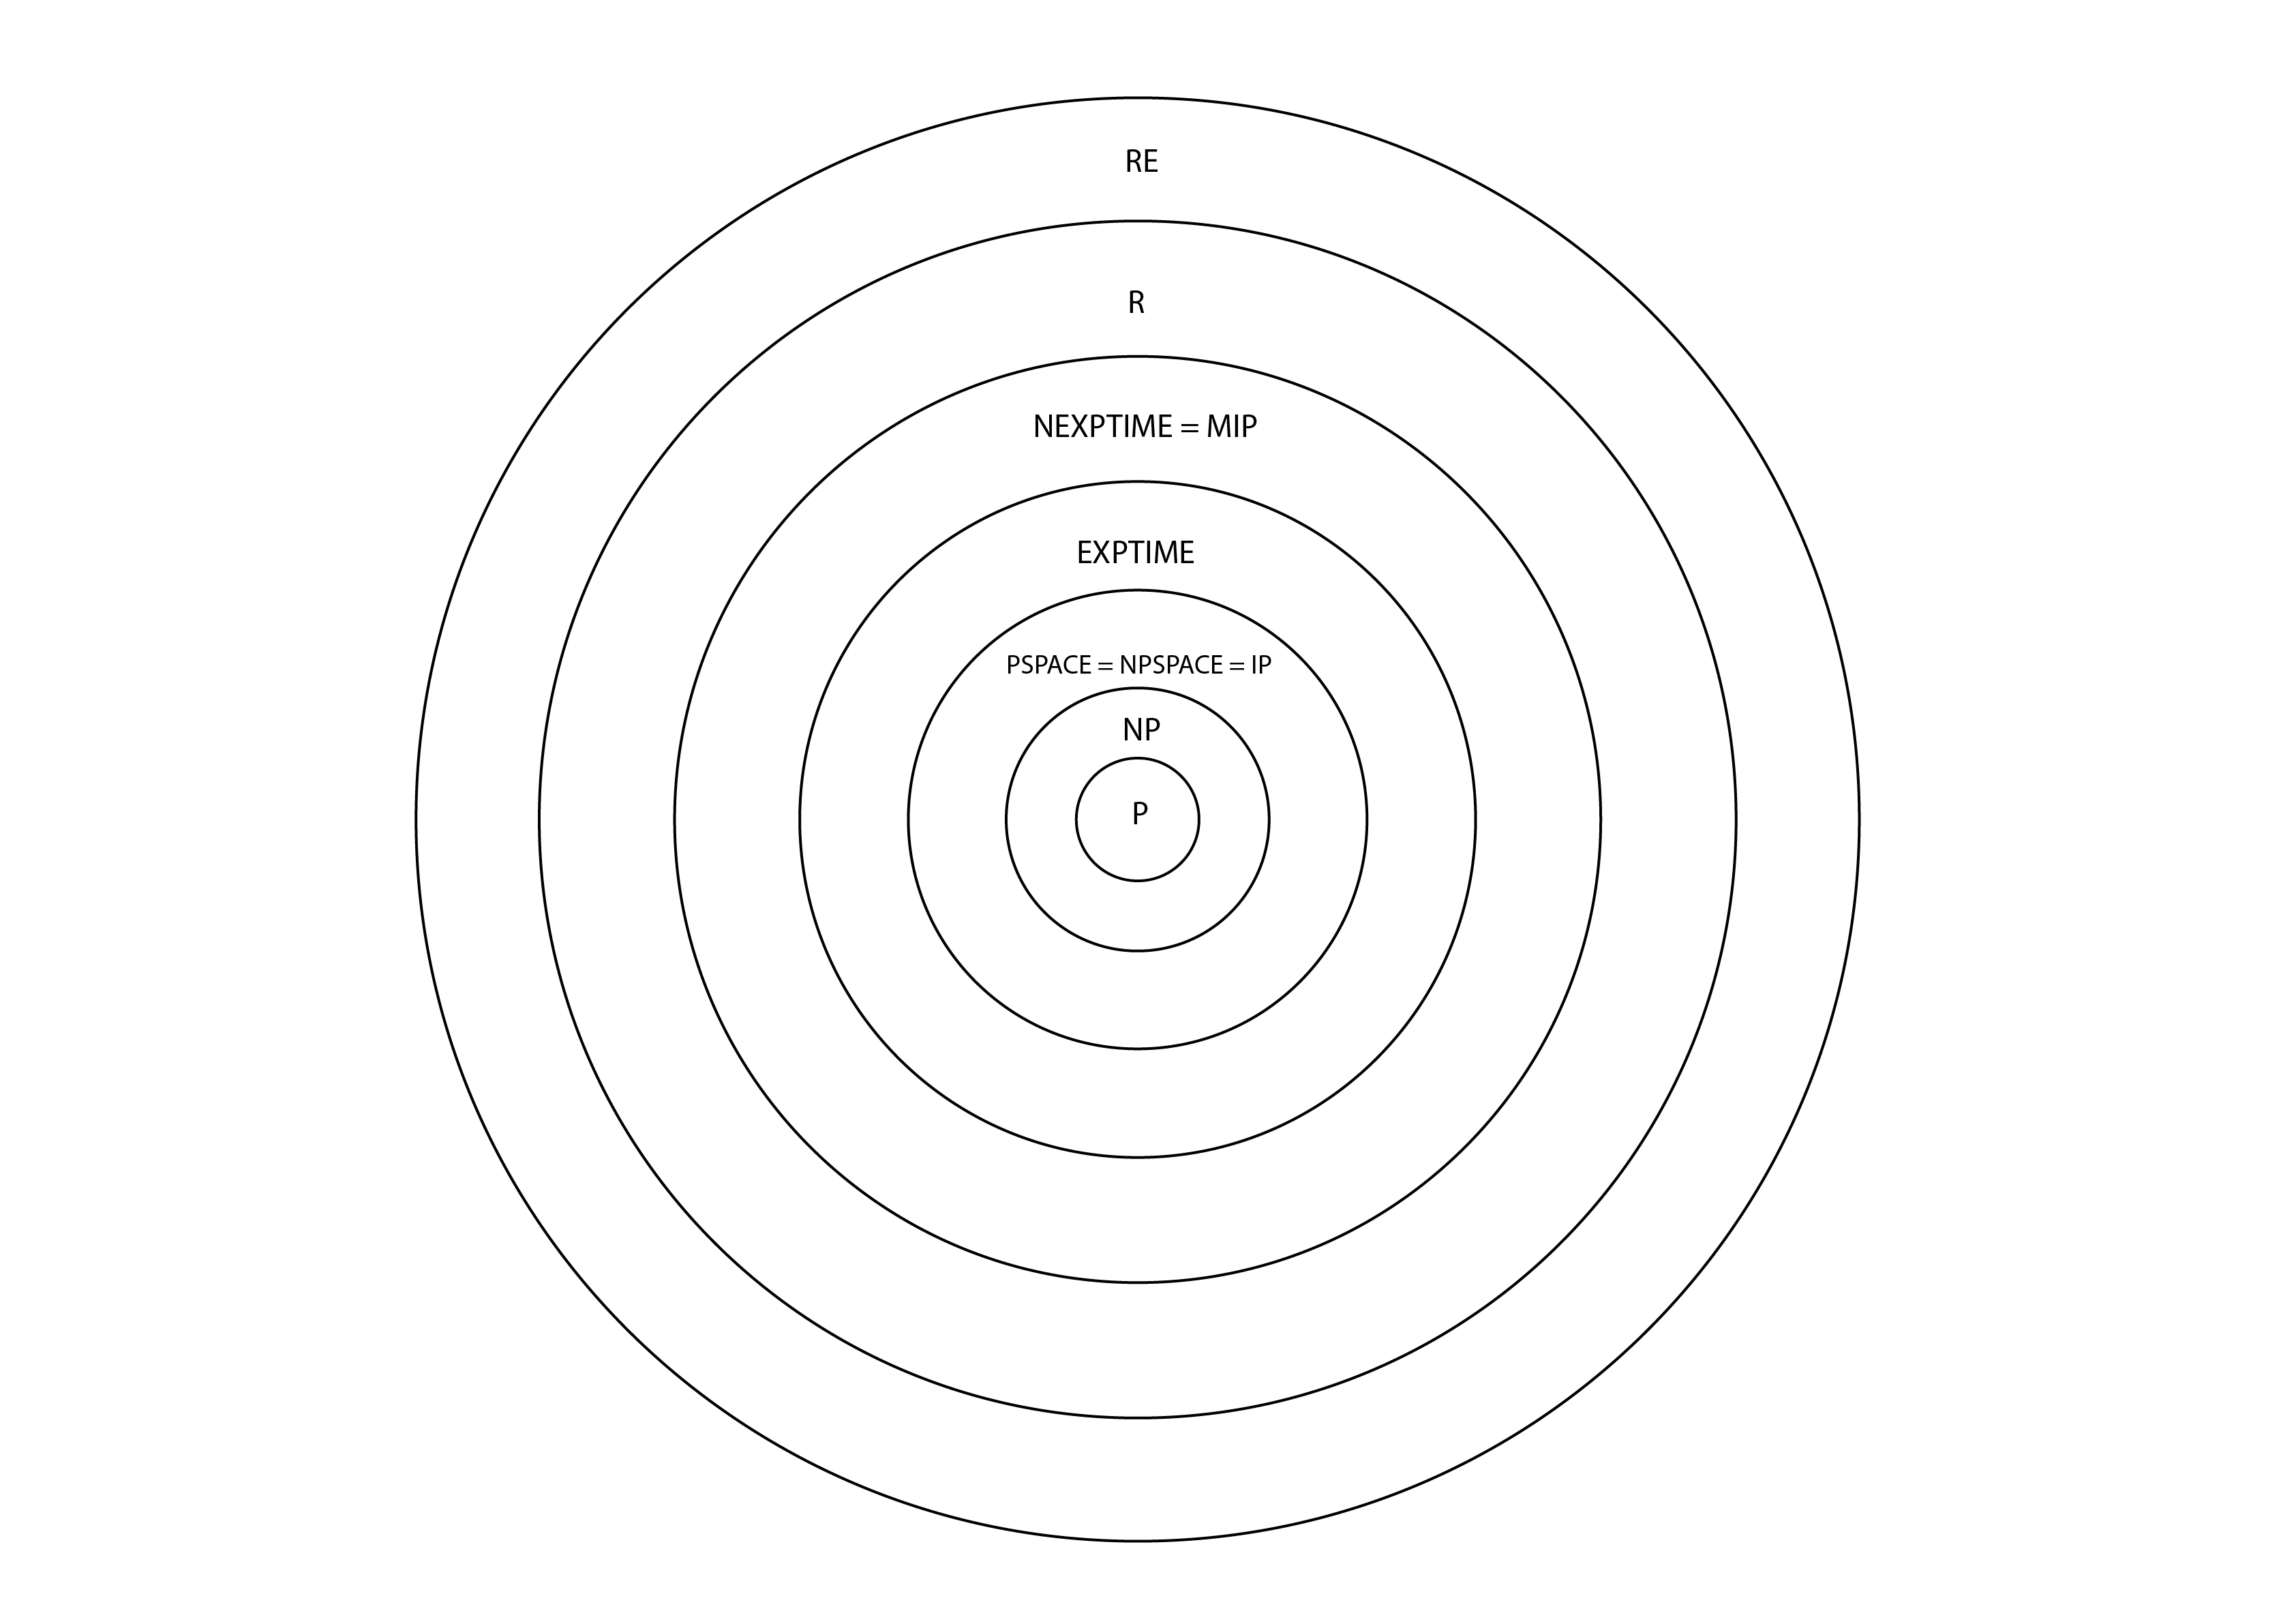
\includegraphics[width=1.1\linewidth]{Complexity.png}
    \centering
    \caption{Complexity classes hierarchy, not in scale.}
    \end{figure}

Given the title of this seminar, it should't been difficult to guess the place of MIP* in the hierarchy, and therefore how much powerful multiprover interactive proof with entanglement are.

